
% ===========================================================================
% Title:
% ---------------------------------------------------------------------------
% to create Type I fonts type "dvips -P cmz -t letter <filename>"
% ===========================================================================
\documentclass[11pt]{article}       %--- LATEX 2e base
\usepackage{latexsym}               %--- LATEX 2e base
%---------------- Wide format -----------------------------------------------
\textwidth=6in \textheight=9in \oddsidemargin=0.25in
\evensidemargin=0.25in \topmargin=-0.5in
%--------------- Algorithm --------------------------------------------------
\newtheorem{algX}{Algorithm}
\newenvironment{algorithm}       {\begin{algX}\begin{em}}%
                                 {\par\noindent --- End of Algorithm ---
                                 \end{em}\end{algX}}
\newcommand{\step}[2]            {\begin{list}{}
                                  {  \setlength{\topsep}{0cm}
                                     \setlength{\partopsep}{0cm}
                                     \setlength{\leftmargin}{0.8cm}
                                     \setlength{\labelwidth}{0.7cm}
                                     \setlength{\labelsep}{0.1cm}    }
                                  \item[#1]#2    \end{list}}
                                 % usage: \begin{algorithm} \label{xyz}
                                 %        ... \step{(1)}{...} ...
                                 %        \end{algorithm}
%--------------- Figures ----------------------------------------------------
\usepackage{graphicx}

\newcommand{\includeFig}[3]      {\begin{figure}[htb] \begin{center}
                                 \includegraphics
                                 [width=4in,keepaspectratio]
                                 {#2}\caption{\label{#1}#3} \end{center} \end{figure}}
                                 % usage: \includeFig{label}{file}{caption}


% ===========================================================================
\begin{document}
% ===========================================================================

% ############################################################################
% Title
% ############################################################################

\title{Accelerating Genetic ANN Training using the CUDA Platform}


% ############################################################################
% Author(s) (no blank lines !)
\author{
% ############################################################################
Catalin Patulea and Robert Peace\\
School of Systems and Computer Engineering\\
Carleton University\\
Ottawa, Canada K1S 5B6\\
{\em rpeace@sce.carleton.ca}
% ############################################################################
} % end-authors
% ############################################################################

\maketitle

% ############################################################################
% Abstract
% ############################################################################
\begin{abstract}
We present an implementation of genetic algorithm (GA) training of artificial neural networks (ANNs) targeting commodity graphics cards (GPUs). By carefully mapping the problem onto the unique GPU architecture, we achieve order-of-magnitude speedup over a conventional CPU implementation. Furthermore, we show that the speedup is consistent across a wide range of population and training set sizes. This performance boost enables classifier design to span a wider range of population sizes and number of generations affording better classifiers and improved understanding of long-term trends in genetic algorithm convergence. Finally, we demonstrate this method in the context of the 2009 UC San Diego Data Mining Contest.
\end{abstract}

% ############################################################################
\section{Introduction} \label{intro}
% ############################################################################

% ############################################################################
\section{Background} \label{background}
% ############################################################################

% ----------------------------------------------------------------------------
\subsection{Artificial Neural Networks} \label{ann}
% ----------------------------------------------------------------------------
Artificial neural networks (ANNs) are very flexible classifiers. By varying the network structure and parameters thereof, they can represent many aspects of the function to be approximated, including nonlinearities and high-order terms. However, the complexity of these classifiers implies that finding optimal parameters is a search in a very high-dimensional parameter space. This is known as an optimization problem, for which a wide variety of solutions are known.

Some approaches to ANN training include gradient descent, Gauss--Newton and Levenberg-�Marquardt. Greedy approaches such as these seek extrema using the local behaviour of the error function and are thus susceptible to getting stuck at local extrema rather than finding the global extremum. Stochastic approaches asymptotically explore the entire search space, offering the promise of "eventually" reaching the global extremum.

% ----------------------------------------------------------------------------
\subsection{Genetic Algorithms} \label{ga}
% ----------------------------------------------------------------------------
Genetic algorithms (GAs) rely on multiple candidate solutions to simultaneously explore the search space. The "individuals" are randomly mutated, mated and selected during each of several generations. Mutation and mating is done using a problem-specific representation of candidate solutions and "genetic operators." Selection is governed by a fitness function (classifier performance). The competitive bias imposed by selection attempts to mimic the "survival of the fittest" principle so often seen in Nature.

GA training of ANNs is very computationally-intensive. For each generation ($10^1$--$10^2$) individuals), the fitness of each individual is calculated by applying each neural network to the entire training set ($10^2$--$10^6$ instances) and taking the classification accuracy for that network. Each ANN evaluation itself requires a large number of multiplications (which increases with the number of features and hidden nodes) in addition to evaluation of transcendentals for the more common node activation functions. Thus, a CPU implementation of GA training of ANNs for any but the smallest networks and training sets is infeasible.

% ----------------------------------------------------------------------------
\subsection{The CUDA Platform} \label{cuda}
% ----------------------------------------------------------------------------
NVidia's Compute Unified Device Architecture (CUDA) is a programming paradigm for massively parallel processors present in off-the-shelf graphics cards (GPUs). GPUs consist of many independent floating-point units, providing significant speedup to data-parallel compute-intensive applications. Each unit is connected to on-board memory using a very wide bus, enabling very high memory bandwidth provided certain particular memory access rules are respected. The combination of these features makes CUDA an ideal platform for GA-ANN training.

The computational unit in CUDA is the "kernel", which is a C function executed in parallel on the grid of available compute units in the CUDA device. The function can request its position in this grid such that it can apply the same algorithm to values at different addresses in memory. In addition, if groups of kernels access sequential addresses in memory, the memory fetches are done in parallel, maximizing bus bandwidth utilization. This is referred to as coalesing.

The CUDA programming model defines global and shared memory. Global memory is on-board but off-chip, expensive for random access and plentiful (100s of MB). Shared memory is on-chip, very fast for random access but very limited (16 KB).

% ----------------------------------------------------------------------------
\subsection{Data Mining Contest} \label{contest}
% ----------------------------------------------------------------------------
The data for our classifier was provided by the 2009 UC San Diego Data Mining Contest "E-commerce Transaction Anomaly Classification" and consist of 94682 instances of 19 features with a 1:50 class imbalance. The evaluation metric was "lift at 20\%", which can be understood as the ratio of the true positive rate in the top 20\% of instances ranked by the classifier to the overall positive rate of the original data set. This metric was directly used as the fitness of each classifier being evaluated by the GA. ANN outputs are treated as confidence values and used for ranking.

% ############################################################################
\section{Methods} \label{algimp}
% ############################################################################
The training process can be divided in several parts which are repeated for each generation until sufficient classifier performance is obtained.
\begin{enumerate}
	\item Genetic algorithm processing -- initialization, mating, mutation, selection
	\item Computation of ANN outputs
	\item Calculation of top 20\% threshold value (each individual)
	\item Counting of the positive instances with outputs above this threshold (each individual)
\end{enumerate}

Item 1 is not very computationally intensive and was not parallelized. Items 2, 3 and 4 were all implemented on the CUDA platform. Performance results are given as the combined time for one generation of these last three items but exclude one-time initialization.

% ----------------------------------------------------------------------------
\subsection{Preliminary Data Analysis} \label{prelim}
% ----------------------------------------------------------------------------
Filling this with text so that I can see what the document looks like when it is filled with text and to make sure that everything lines up nicely when it is full of text like this

% ----------------------------------------------------------------------------
\subsection{Data Preprocessing Steps} \label{preprocessing}
% ----------------------------------------------------------------------------
Filling this with text so that I can see what the document looks like when it is filled with text and to make sure that everything lines up nicely when it is full of text like this

% ----------------------------------------------------------------------------
\subsection{Classifier Design} \label{design}
% ----------------------------------------------------------------------------
Filling this with text so that I can see what the document looks like when it is filled with text and to make sure that everything lines up nicely when it is full of text like this

% ----------------------------------------------------------------------------
\subsection{Classifier Implementation} \label{implementation}
% ----------------------------------------------------------------------------
Filling this with text so that I can see what the document looks like when it is filled with text and to make sure that everything lines up nicely when it is full of text like this

% ----------------------------------------------------------------------------
\subsection{Computation of ANN Output Values} \label{implementation}
% ----------------------------------------------------------------------------
ANN output values are computed by reading feature values and applying the appropriate operations represented by the network topology and parameters. Feature data are organized to enable memory read coalescing. This part of the process is particularly well-suited to the CUDA architecture because it has a very high ratio of mathematical operations to memory accesses (160 multiplications, 4 exponentiations and 80 bytes of memory accesses for our ANN topology).

% ----------------------------------------------------------------------------
\subsection{Calculation of Top 20\% Threshold} \label{implementation}
% ----------------------------------------------------------------------------
To efficiently calculate the top 20\% threshold in a list of $n$ ANN output values, we can insert all values into a $k$-sized minheap where $k = 0.20 * n$, and take the root of the heap as the threshold. Each minheap insertion costs $O(\log k)$ time. Because device shared memory (16~KB) is not large enough for our value of $k$, we use $p$ passes of $\frac{k}{p}$-sized heaps with which we find the top 5\% threshold, then the top 10\%, etc. The overall complexity of our algorithm is $O(np \log \frac{k}{p})$. Parallelization is across individuals.

% ----------------------------------------------------------------------------
\subsection{Counting of Positives Above Threshold} \label{implementation}
% ----------------------------------------------------------------------------
By keeping positive instances first in our training set, we avoid the need to consult the class of each instance (saving a costly global memory read). We simply iterate over the first $numPositives$ ANN outputs and count the outputs over the individual's 20\% threshold. Parallelization is across both individuals and groups of outputs. For each individual, we keep m counters which accumulate counts for indexes $i$ where $i \equiv 0 \bmod{m}$, $i \equiv 1 \bmod{m}$, ..., $i \equiv m - 1 \bmod{m}$. This enables parallelization even when there are not enough individuals in the population to fully occupy the device. Each batch of $m$ kernels accesses $m$ sequential locations in memory, which results in coalesced reads.

% ############################################################################
\section{Results} \label{results}
% ############################################################################
Filling this with text so that I can see what the document looks like when it is filled with text and to make sure that everything lines up nicely when it is full of text like this

% ----------------------------------------------------------------------------
\subsection{Experimental Setup} \label{experiment}
% ----------------------------------------------------------------------------
To evaluate the performance of our system, we compared execution time of equivalent algorithms running on commodity desktop CPUs and GPUs. Each series represents one type of experimental hardware (Table~\ref{tab:experimental-hardware}). Each data point is an average over 10 runs of the algorithm with the same parameters.

\begin{table}
	\centering
	\begin{tabular}{ll}
	\textbf{Legend Label} & \textbf{Hardware} \\
	\hline
	Core2 & Intel Core 2 Q9450 CPU at 2.66 GHz \\
	GTX275 & NVidia GTX275 GPU \\
	\hline
	\end{tabular}
	\caption{Experimental hardware}
	\label{tab:experimental-hardware}
\end{table}

% ----------------------------------------------------------------------------
\subsection{Performance Results} \label{performance}
% ----------------------------------------------------------------------------
In most cases, the GPU implementation resulted in approximately an order of magnitude speedup over a CPU implementation (Figure~\ref{fig:training-performance}). For low population sizes, GPU initialization and data copying dominates.

\begin{figure}
	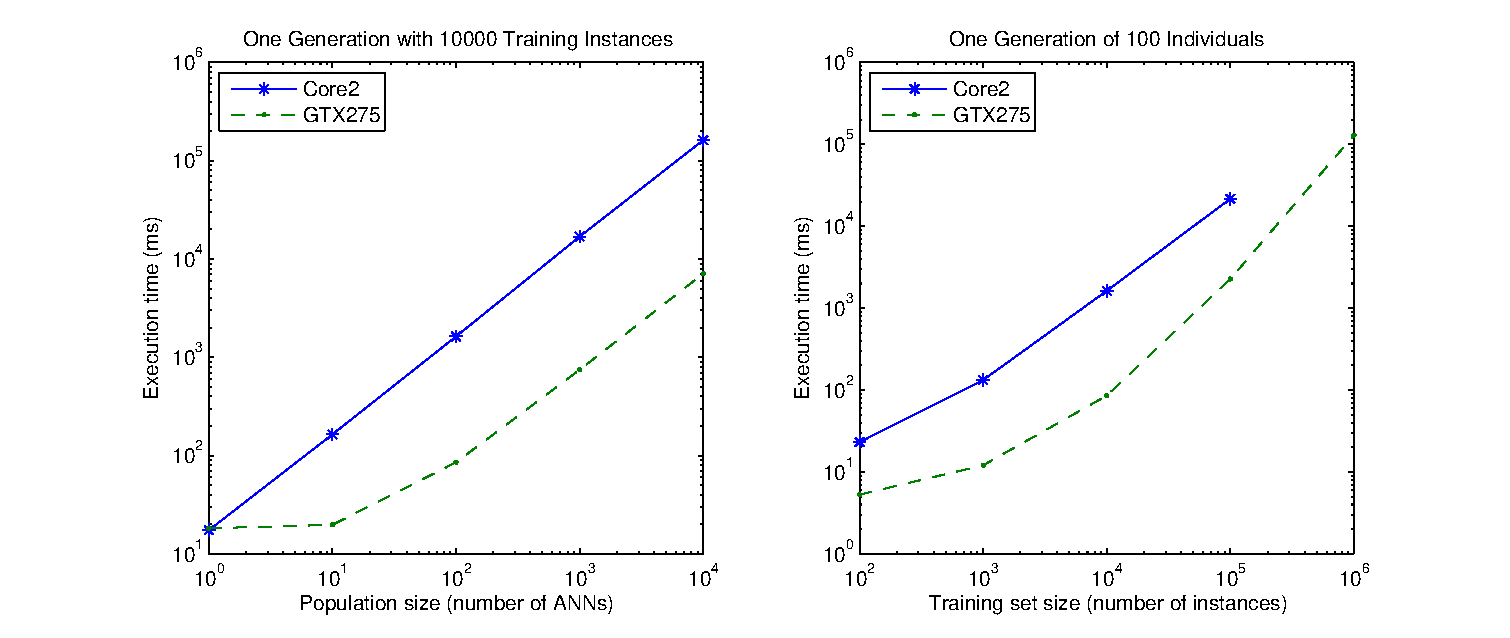
\includegraphics[width=\textwidth]{fig-performance}
	\caption{Training performance as a function of population size (left) and training set size (right). Note logarithmic axes.}
	\label{fig:training-performance}
\end{figure}

% ----------------------------------------------------------------------------
\subsection{Classifier Results} \label{results}
% ----------------------------------------------------------------------------
Filling this with text so that I can see what the document looks like when it is filled with text and to make sure that everything lines up nicely when it is full of text like this

% ############################################################################
\section{Conclusion} \label{concl}
% ############################################################################
We have presented an implementation of GA training of ANN classifiers for the CUDA platform for GPU programming. By carefully designing memory organization, algorithm computational load and memory access patterns, we have obtained a 10-fold speedup compared to a conventional sequential CPU implementation. Additional workaround were necessary for the low amount of fast on-chip GPU memory. Our method scales across population and training set sizes.

% ############################################################################
\section{Discussion} \label{disc}
% ############################################################################
Filling this with text so that I can see what the document looks like when it is filled with text and to make sure that everything lines up nicely when it is full of text like this

% ----------------------------------------------------------------------------
\subsection{Future Work} \label{future}
% ----------------------------------------------------------------------------
Filling this with text so that I can see what the document looks like when it is filled with text and to make sure that everything lines up nicely when it is full of text like this

% ############################################################################
% Bibliography
% ############################################################################
\bibliographystyle{plain}
\bibliography{bibliography}     %loads bibliography.bib

% ============================================================================
\end{document}
% ============================================================================
